\documentclass{article}

\usepackage[utf8]{inputenc}
\usepackage[T1]{fontenc}
\usepackage{hyperref}
\usepackage{geometry}
\usepackage{graphicx}
\usepackage{multirow}
\usepackage{hhline}
\usepackage{makecell}
\usepackage{subcaption}
\usepackage[english]{babel}

\hypersetup{
	colorlinks=true, %set true if you want colored links
	linktoc=all,     %set to all if you want both sections and subsections linked
	linkcolor=blue,  %choose some color if you want links to stand out
}

\geometry{
	a4paper,
	left=10mm,
	right=10mm,
	top=10mm,
	bottom=10mm,
}

\newcommand{\tabitem}{~~\llap{\textbullet}~~}
\addto\captionsenglish{\renewcommand{\figurename}{Gambar}}

\begin{document}

\begin{table}[!ht]
	\centering
	\begin{tabular}{|l|l|l|l|}
		\hline
		\multirow{3}{*}{
\includegraphics[width=0.25\columnwidth]{logoviblab}} & \multicolumn{3}{l|}{\makecell{\textbf{MINUTES OF MEETING}}} \\
		\cline{2-4}
		& \textbf{Location of Meeting} & \textbf{Time/Date of Meeting} & \textbf{Date of this Report}  \\
		\cline{2-4}
		& \makecell{PT Global Quality Indonesia \\
		KOPO MAS REGENSI \\
		BLOK N - No. 7 C \\
		Bandung-Indonesia} & \makecell{9 Februari 2023 \\ 11:00 WIB} & 13 Februari 2023\\
		\hline
		\multicolumn{4}{|l|}{\textbf{Subject:}} \\
		\hline
		\multicolumn{4}{|l|}{Diskusi Awal Pengujian Unit Audiometri} \\
		\hline
		\multicolumn{2}{|l|}{\textbf{Attendees:}} & \multicolumn{2}{l|}{\textbf{Distribution}} \\
		\hline
		1. Achmadi, ST MT & ITS & & \\
		\hline
		2. Elliyana Firmansyah & PT GQI & & \\
		\hline
		\makecell[l]{3. Mas Ahmad \\(asisten Pak Elliyana)} & PT GQI & & \\
		\hline

		\multicolumn{4}{|l|}{\textbf{Minuted by: Achmadi ST MT}} \\
		\hline

		\multicolumn{3}{|l|}{\textbf{Discussion}}& \textbf{Action By} \\
		\hline
		\multicolumn{3}{|l|}{\makecell[l]{
				Parameter Audiometri dari Kemenkes yang akan diuji: \\
				\tabitem Hearing Level (Air Conduction) \\
				\tabitem Bone Conduction \\
				\tabitem Frequency \\}} & Info \\
		\hline
		\multicolumn{3}{|l|}{\makecell[l]{
				Parameter Audiometri yang bisa diuji: \\
				\tabitem Hearing Level (Air Conduction)\\
		Pengukuran menggunakan SLM seperti kebisingan Industri}} & PT GQI \\
		\hline
		\multicolumn{3}{|l|}{\makecell[l]{
				Parameter Uji Fisik: \\
				\tabitem Safety casing untuk penggunaan \\
				\tabitem Electrical Safety \\
				\tabitem Mengikuti Manual \\}} & PT GQI \\
		\hline
		\multicolumn{3}{|l|}{\makecell[l]{
				Parameter Uji Fungsi: \\
				\tabitem Fungsi Tombol \\
				\tabitem Fungsi Display \\
				\tabitem Mengikuti Manual \\}} & PT GQI \\
		\hline
		\multicolumn{3}{|l|}{\makecell[l]{
				Catatan Penting: \\
				\tabitem Tidak semua prosedur sudah ter-KAN \\
				\tabitem Audiometri termasuk belum KAN \\
				\tabitem Laporan PT QGI dapat mempermudah uji BPFK \\}} & Info \\
		\hline
	\end{tabular}
\end{table}

\begin{figure}[!ht]
	\centering
	\begin{subfigure}[t]{0.45\textwidth}
		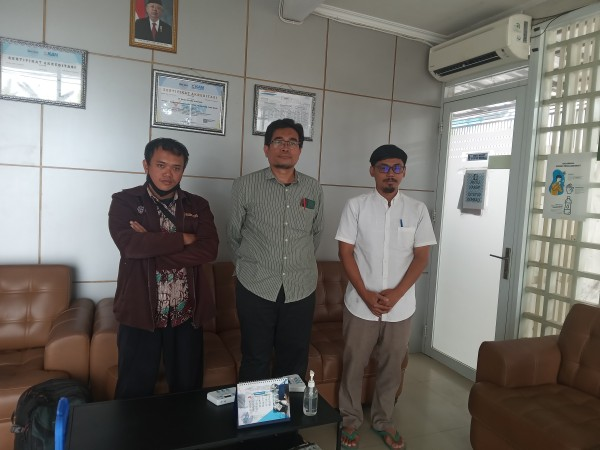
\includegraphics[width=\textwidth]{dokumentasi/rapat}
		\caption{Pertemuan}
	\end{subfigure}
	\begin{subfigure}[t]{0.45\textwidth}
		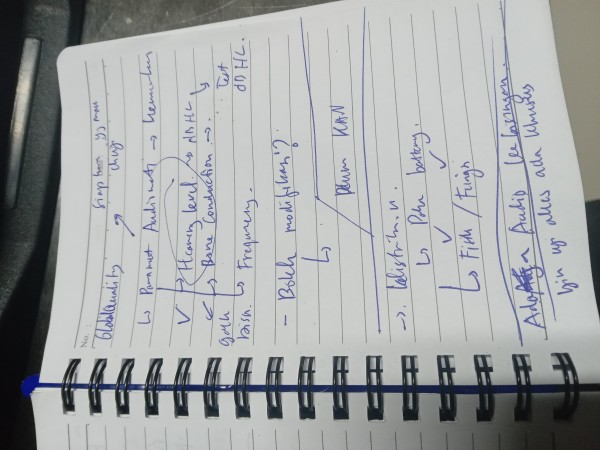
\includegraphics[width=\textwidth]{dokumentasi/catatan}
		\caption{Catatan}
	\end{subfigure}
	\\

	\caption{Dokumentasi}
\end{figure}

\end{document}
